
\chapter{System analysis}

This chapter is about analyzing the to be implemented system more detailed, separating concerns\todo{cite?} and starting to evaluate solutions in an architectural viewpoint.
It is important to find an architecture, that is able to fulfill all requirements and is able to be evolved on for upcoming needs.
In some areas where this is foreseeable, preparations can be implemented, whereas in other regions this is not possible.
When working on a architecture, the SOLID\todo{.} and YAGNI\todo{.} principles can help to evaluate the stability and expandability\todo{can it?}.



\pagebreak
\section{System Architecture}

In \autoref{architecture:detailed} a high level overview of the architecture is shown.
It shows various services and regions with internal and external communication channels.
The architecture follows the \enquote{Onion Architecture Pattern}\todo{cite}, which is also indicated by the layer numbers and coloring (inner layers are darker).


\begin{figure}[H]
	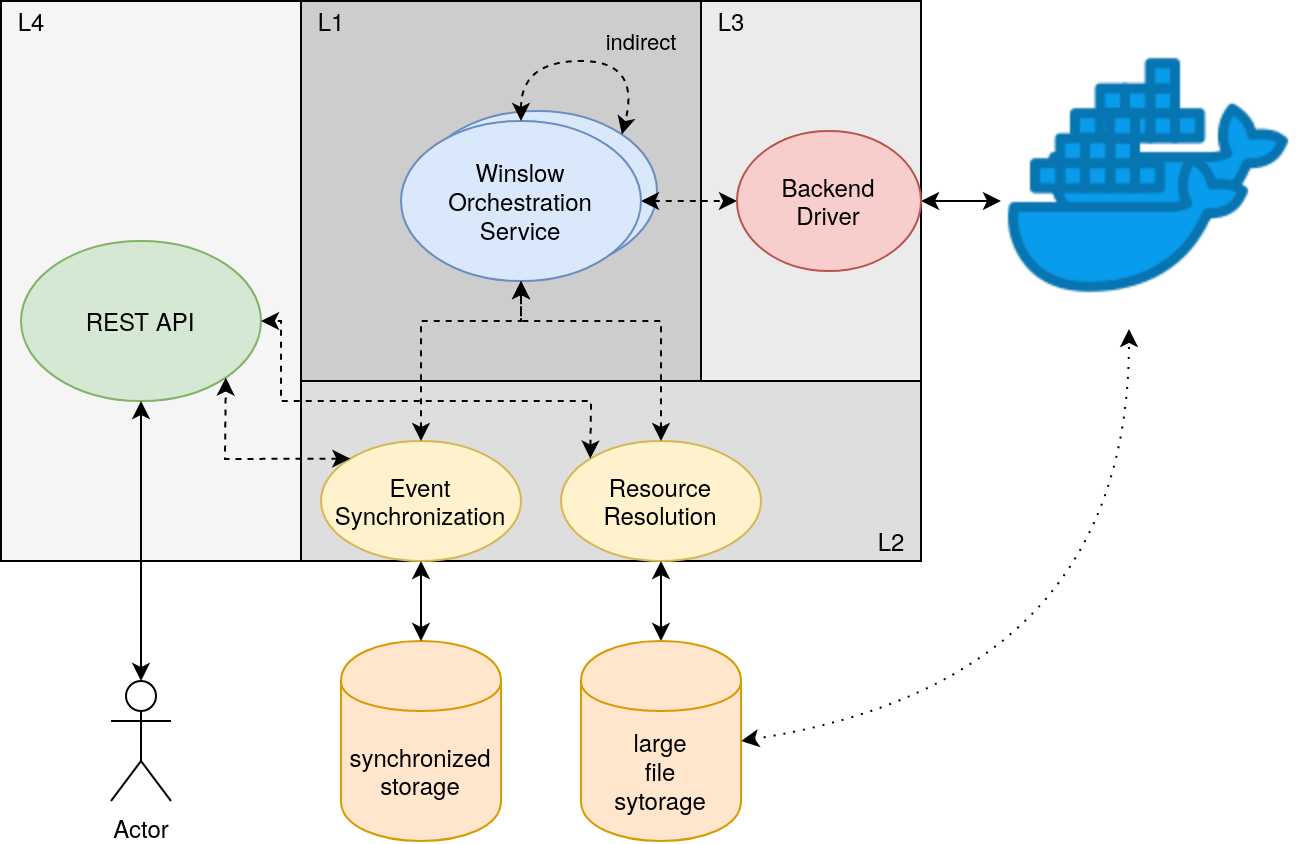
\includegraphics[width=0.99\textwidth]{architecture_detailed.png}
	\centering
	\caption{Architecture overview of a Winslow instance}
	\label{architecture:detailed}
\end{figure}

The meaning of the layers and their services will be explained in the following sub-sections.

\subsection{Layer 1: Orchestration Service}

This layer is all about the fundamental business logic: when to schedule, start and fail which stage of what project, while watching the hardware utilization.
This level is also responsible to coordinate these actions between all Winslow instances, so that there is no duplicate, missing or undetected node failure.

The following requirements are therefore implemented here: \todo{.?}

\subsection{Layer 2: Events and Resources}
\label{architecture:layer:event_bus}

For the first layer to communicate with the environment, such as reading configurations, project files or cooperation commands, this layer is essential.
It provides two important services: a synchronized event bus and a large file resource management.
The first is used to communicate with the other Winslow instances, while the latter is required for a stage execution.
Although list here as two separate services, they do not necessarily need to be backed up by two storages.
To provide a synchronized stream of events, it is required that the underlying storage provides some sort of synchronization primitives (see \todo{ref stream api / files?}).
The large file storage has no such requirement, as this is ensured by Winslow's stage synchronization and thus a eventual consistent\todo{cite} storage could be used here.

While knowing the different requirements, because of the time constraint of this thesis, a common NFS storage will be used\todo{autoref}.

\subsection{Layer 3: Backend Driver}

This layer is responsible to bind a remote or external service to the reach of Winslow.
Once the orchestration service decided to run a stage, collected all environment variables and prepared the workspace, the backend driver is instructed to start a certain image with said prepared environment.
By separating this task to its own layer - and service in this case - it will be easier to change from Docker to another platform if necessary.
A reason for this could be the change of needs, the appearance of a platform that is fulfilling the needs better or the disappearance of the currently used platform.
The latter sounds not that common at first, but the recent partial acquisition of Docker Inc by Mirantis\cite{docker:acquisition} proves that even very popular third party software is not going to be around for all eternity.
By moving the driver implementation into its own layer, but leaving the interface definition in layer 1, this also complies to the \enquote{Dependency Inversion Principle}. \todo{.}

While the backend driver does not access any storage itself, the stages need to read and write to the large file storage.
In the case of the Docker implementation with an NFS share, the access from within the executed stage can be guarded to limit read and write access to only the required working directories.
This is discussed more in-depth in \todo{autoref}.

\subsection{Layer 4: Client Communication}

The final layer in this architecture is the client communication layer.
This service is not crucial for the actual execution and may be disabled on Winslow instances that shall not response to a user input themselves.
The REST API\todo{autoref rest} provides sites that can be called from the static Angular\todo{autref angular} content to upload or download files, to control stage execution and to monitor usage and logs.
Removing or disabling this layer is not stopping the Winslow

\begin{comment}
\section{Use Case Diagrams}
Finding all requirements can be challenging.
Drawing Use Case Diagrams can help to discover requirements while being very easy to understand.
This helps in understanding the customers needs \cite{Rosenberg2007} while the customer receives an impression on what will be reflected in the final product.

Listing all use cases in a single diagram negates the desired effect of it being easily understandable because of the number of interaction possibilities.
Instead, the interactions are grouped in categories and displayed in separate diagrams.
\autoref{use_case:overview} shows high-level use cases of all categories that are relevant to a user of the system.

\begin{figure}[H]
	\scalebox{.65}{
		\begin{tikzpicture}[node distance=5]
		\begin{umlsystem}{Winslow - Interaction Categories}
		\umlusecase[y=0,name=u1]{Manage Pipelines and Projects [\autoref{use_case:mgmt}]}
		\umlusecase[y=-1,name=u2]{Manage Resources and Workspaces [\autoref{use_case:files}]}
		\umlusecase[y=-2,name=u3]{Manage and Monitor Execution [\autoref{use_case:execution}]}
		\umlusecase[y=-3,name=u4]{Monitor Nodes [\autoref{use_case:monitor}]}
		\end{umlsystem}
		\umlactor[x=-9.5,y=-1.5]{User}
		\umlassoc{User}{u1}
		\umlassoc{User}{u2}
		\umlassoc{User}{u3}
		\umlassoc{User}{u4}
		\end{tikzpicture}
	}
	\centering
	\caption{Use Case Diagram showing the top level interaction categories}
	\label{use_case:overview}
\end{figure}

\subsection{Managing Pipelines and Projects}
\label{use_case:mgmt}

\todo{.}

\begin{figure}[H]
	\scalebox{.65}{
		\begin{tikzpicture}[node distance=5]
		\begin{umlsystem}{Winslow - Manage Pipelines and Projects}
		\umlusecase[y=0,name=u110]{\reqNameRef{mgmt:create:pipeline}}
		\umlusecase[y=-1,name=u120]{\reqNameRef{mgmt:update:pipeline}}
		\umlusecase[y=-2,name=u130]{\reqNameRef{mgmt:delete:pipeline}}
		\umlusecase[y=-3,name=u140]{\reqNameRef{mgmt:list:pipeline}}
		
		\umlusecase[y=-5,name=u210]{\reqNameRef{mgmt:create:project}}
		\umlusecase[y=-6,name=u220]{\reqNameRef{mgmt:update:project:pipeline}}
		\umlusecase[y=-7,name=u230]{\reqNameRef{mgmt:update:project:name}}
		\umlusecase[y=-8,name=u240]{\reqNameRef{mgmt:update:project:labels}}
		\umlusecase[y=-9,name=u250]{\reqNameRef{mgmt:delete:project}}
		\umlusecase[y=-10,name=u260]{\reqNameRef{mgmt:list:project}}
		\end{umlsystem}
		\umlactor[x=-9.5,y=-4]{User}
		\umlassoc{User}{u110}
		\umlassoc{User}{u120}
		\umlassoc{User}{u130}
		\umlassoc{User}{u140}
		\umlassoc{User}{u210}
		\umlassoc{User}{u220}
		\umlassoc{User}{u230}
		\umlassoc{User}{u240}
		\umlassoc{User}{u250}
		\umlassoc{User}{u260}
		\end{tikzpicture}
	}
	\centering
	\caption{Use Case Diagram showing the general management interactions}
\end{figure}


\subsection{Managing Resources and Workspaces}
\label{use_case:files}

\todo{.}

\begin{figure}[H]
	\scalebox{.65}{
		\begin{tikzpicture}[node distance=5]
		\begin{umlsystem}{Winslow - Manage Resources and Workspaces}
		\umlusecase[y=0,name=u110]{\reqNameRef{files:upload}}
		\umlusecase[y=-1,name=u120]{\reqNameRef{files:download}}
		\umlusecase[y=-2,name=u130]{\reqNameRef{files:list}}
		\end{umlsystem}
		\umlactor[x=-9.5,y=-1]{User}
		\umlassoc{User}{u110}
		\umlassoc{User}{u120}
		\umlassoc{User}{u130}
		\end{tikzpicture}
	}
	\centering
	\caption{Use Case Diagram showing the general management interactions}
\end{figure}

\subsection{Managing and Monitoring Executions}
\label{use_case:execution}

\todo{.}

\begin{figure}[H]
	\scalebox{.65}{
		\begin{tikzpicture}[node distance=5]
		\begin{umlsystem}{Winslow - Manage and Monitor Executions}
		\umlusecase[y=0,name=u110]{\reqNameRef{exec:start:stage}}
		\umlusecase[y=-1,name=u120]{\reqNameRef{exec:pause:stage}}
		\umlusecase[y=-2,name=u130]{\reqNameRef{exec:resume:stage}}
		\umlusecase[y=-3,name=u140]{\reqNameRef{exec:abort:stage}}
		\umlusecase[y=-5,name=u150]{\reqNameRef{exec:inspect:logs}}
		\umlusecase[y=-6,name=u160]{\reqNameRef{exec:inspect:state}}
		\end{umlsystem}
		\umlactor[x=-9.5,y=-3]{User}
		\umlassoc{User}{u110}
		\umlassoc{User}{u120}
		\umlassoc{User}{u130}
		\umlassoc{User}{u140}
		\umlassoc{User}{u150}
		\umlassoc{User}{u160}
		\end{tikzpicture}
	}
	\centering
	\caption{Use Case Diagram showing the general management interactions}
\end{figure}

\subsection{Monitoring Nodes}
\label{use_case:monitor}
\todo{.}
\begin{figure}[H]
	\scalebox{.65}{
		\begin{tikzpicture}[node distance=5]
		\begin{umlsystem}{Winslow - Monitor Nodes}
		\umlusecase[y=0,name=u110]{\reqNameRef{node:monitor:cpu}}
		\umlusecase[y=-1,name=u120]{\reqNameRef{node:monitor:ram}}
		\umlusecase[y=-2,name=u130]{\reqNameRef{node:monitor:netio}}
		\end{umlsystem}
		\umlactor[x=-9.5,y=-1]{User}
		\umlassoc{User}{u110}
		\umlassoc{User}{u120}
		\umlassoc{User}{u130}
		\end{tikzpicture}
	}
	\centering
	\caption{Use Case Diagram showing the general management interactions}
\end{figure}


\subsection{System Administration}

Furthermore to the interactions with a user, the system must provide further capabilities that are \todo{of} concern to the administrator.


\begin{figure}[H]
	\scalebox{.65}{
		\begin{tikzpicture}[node distance=5]
		\begin{umlsystem}{Winslow - Administration}
		\umlusecase[y=0,name=u1]{Start and Add a new Node}
		\umlusecase[y=-2,name=u2]{Stop and Remove a Node}
		\umlusecase[y=-4,name=u3]{Debug behavior of a Node}
		\end{umlsystem}
		\umlactor[x=-9.5,y=-2]{Admin}
		\umlassoc{Admin}{u1}
		\umlassoc{Admin}{u2}
		\umlassoc{Admin}{u3}
		\end{tikzpicture}
	}
	\centering
	\caption{Use Case Diagram showing administrative interactions}
	\label{use_case:admin}
\end{figure}
\end{comment}

\section{Communication / message analysis ?}

For the communication described in \autoref{architecture:layer:event_bus} messages need to be defined.
Because this is a multi instance system which can suffer partial failure, all operations that are non-instantaneous require to have a timeout, so that a failure is detectable.
Without a failure detection, the end of an operation might not be signaled, which could potentially block further operations for ever.

To account for transmission delay and clock offsets an additional time padding is granted. \todo{.}

\todo{all messages are broadcast because of bus}

\todo{all messages have an id}

\todo{to detailed here? move detailed description to system design?}

\begin{itemize}
	\item \textbf{LOCK}: Locking a named resource or operation.
	A lock is exclusive to the issuer and can only be granted if no other lock of the subject or parts of it exist.
	\item \textbf{EXTEND}: Extending an ongoing operation timeout.
	This can be used to signal, that a lock is required although its timeout is closing by, in which case the point in time the timeout is reached is pushed back.
	The issuer must be the same node as the one that issued the \textbf{LOCK} previously.
	\item \textbf{RELEASE}: An operation or resource is no longer required.
	The issuer must be the same node as the one that issued the \textbf{LOCK} previously.
	\item \textbf{KILL}: Non-gracefully stop an operation or destroy a lock.
	This signals that an operation on its own or associated to a lock shall be stopped immediately and that the lock shall be released.
	At the moment, this is only used whenever a user wants cancel a stage execution early. More details in \todo{autoref}.
	\item \textbf{ELECTION\_START}: Signals that the need to execute a stage was detected.
	The project, pipeline and stage execution id this message is about is included.
	\item \textbf{ELECTION\_PARTICIPATE}: Signals that the issuer node is capable of executing the stage.
	It also includes a scoring for the affinity and aversion of executing the stage\todo{cite} on the issuer node.
	This message also includes the id to the \textbf{ELECTION\_START} it refers to.
	\item \textbf{ELECTION\_STOP}: Signals that the election has ended.
	The participator with the best affinity and aversion scoring is now allowed to start to execute the stage.
	More detail in \todo{auref}.
	The issuer must be the same node as the one that issued the \textbf{ELECTION\_START} previously.
\end{itemize}

%\section{Interface analysis}
% huh?